\chapter{Algorithme}


\section{Minimax}

\flushleft Dans une première partie nous nous sommes
intéressés au minmax de profondeur 0, cet algorithme permettait de jouer mais sans récursivité, il
ne fonctionnait donc pas en profondeur 1 et plus. Après avoir réussit à faire cet algorithme, nous
avons travaillé sur l'implémentation de la récursivité de cet algorithme.


Au début nous nous étions précipités sur le jeu, l'implémentation de MinMax était donc incompatible
avec notre jeu. Nous avons donc tout supprimé pour recommencer sur de meilleur base.
Après avoir reprogrammé le jeu de base, l'implémentation de MinMax était plus facile.

Les captures d'écrans suivantes sont des tentatives avant d'arriver au minmax final.
\begin{figure}[!ht]
\begin{center}
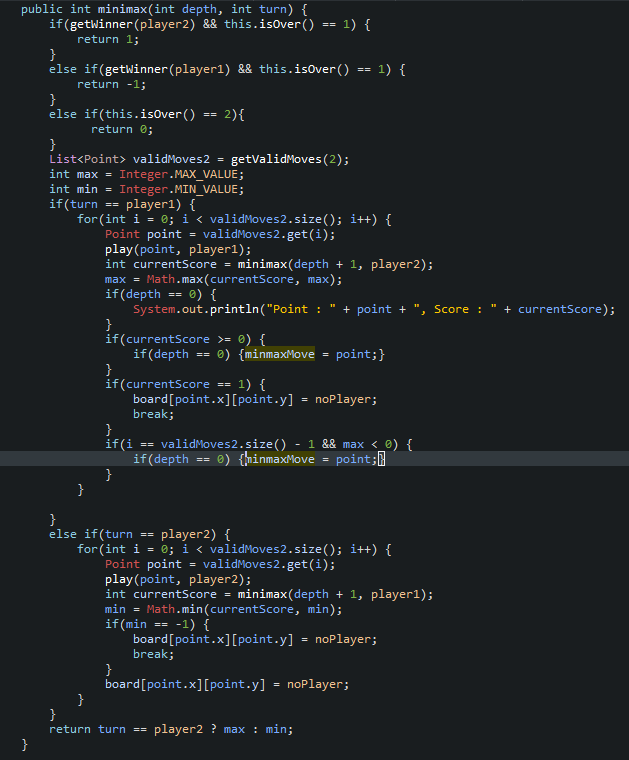
\includegraphics[width=0.65\textwidth]{./MINMAXDEBUT1}
\end{center}
\end{figure}
\newpage

\begin{figure}[!ht]
\begin{center}
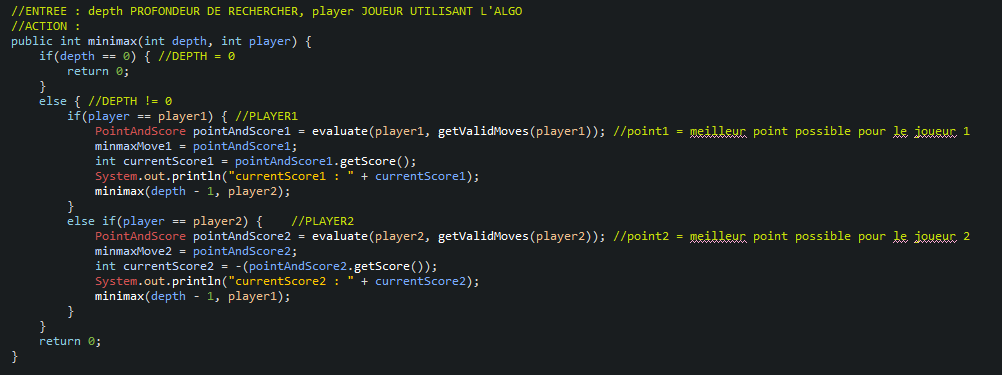
\includegraphics[width=0.85\textwidth]{./MINMAXDEBUT2}
\end{center}
\end{figure}

\centering \textbf{Après avoir vraiment compris l'algorithme en général, et après plusieurs tentatives nous avons
réussit a implémenter l'algorithme et à le debugger.} \\ 


\centering \textbf{La capture d'écran suivante est notre MinMax final.}

\begin{figure}[!ht]
\begin{center}
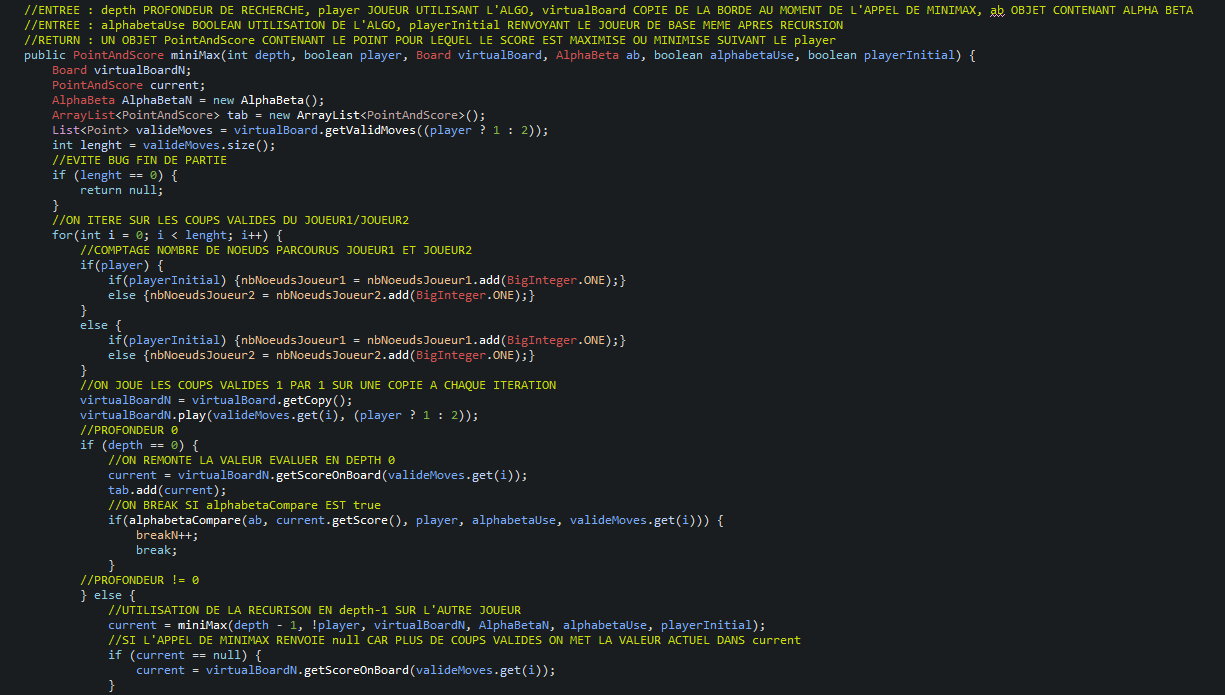
\includegraphics[width=0.95\textwidth]{./MINMAX1} 
\end{center}
\end{figure}

\begin{figure}[!ht]
\begin{center}
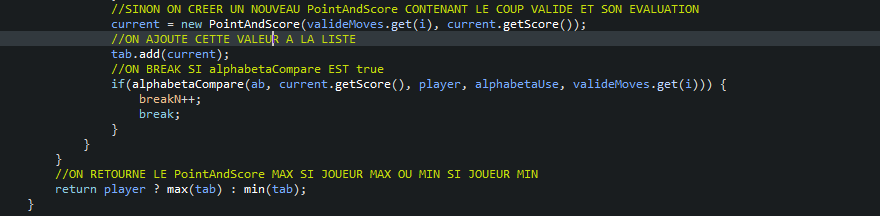
\includegraphics[width=0.75\textwidth]{./MINMAX2}
\end{center}
\end{figure}

\begin{figure}[!ht]
\begin{center}
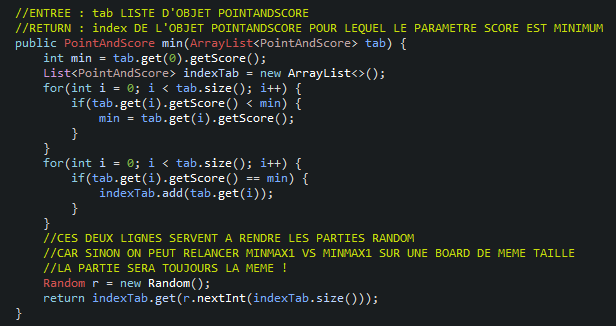
\includegraphics[width=0.65\textwidth]{./MIN}
\end{center}
\end{figure}

\begin{figure}[!ht]
\begin{center}
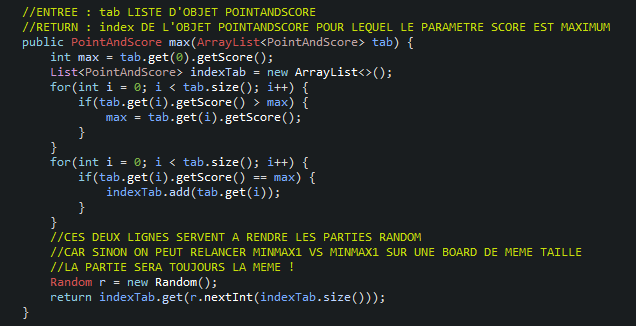
\includegraphics[width=0.65\textwidth]{./MAX}
\end{center}
\end{figure}

\newpage

\section{AlphaBeta}

L'algorithme AlphaBeta semblait plutôt simple après avoir implémenter MinMax.
Nous avons donc essayé de l'implémenter puis de le debugger mais le nombre d'informations
même sur une petite grille et une petite profondeur de minmax rendait le problème complexe.
Après plusieurs tentatives nous n'avons pas réussit à implémenter AlphaBeta.
Le problème étant peu être la structure de MinMax, il y a surement besoin de changer MinMax
afin de pouvoir implémenter AlphaBeta. Le problème semble être lié la récursivité.

\begin{figure}[!ht]
\begin{center}
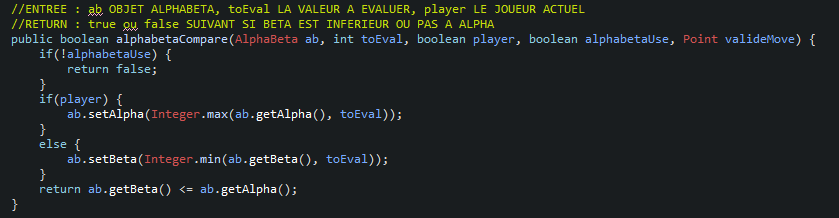
\includegraphics[width=0.90\textwidth]{./ALPHABETA}
\end{center}
\end{figure}

